\documentclass[11pt]{article}

\setlength{\oddsidemargin}{-0.25 in}
\setlength{\evensidemargin}{-0.25 in}
\setlength{\topmargin}{-0.9 in}
\setlength{\textwidth}{7.0 in}
\setlength{\textheight}{9.0 in}
\setlength{\headsep}{0.75 in}
\setlength{\parindent}{0.3 in}
\setlength{\parskip}{0.1 in}
\usepackage{epsf}
\usepackage{pseudocode}
\usepackage[shortlabels]{enumitem}
\usepackage{amsmath}
\usepackage{amssymb}
\usepackage{color}
\usepackage[normalem]{ulem}
\usepackage{graphicx}
\usepackage[export]{adjustbox}
\usepackage{wrapfig}
\pagenumbering{arabic}
\def\O{\mathop{\smash{O}}\nolimits}
\def\o{\mathop{\smash{o}}\nolimits}
\newcommand{\e}{{\rm e}}
\newcommand{\R}{{\bf R}}
\newcommand{\Z}{{\bf Z}}

%% display solutions or not
\newif\ifsol
% \soltrue % comment out to hide solutions

\title{Section 10: Bayes' Nets}
\date{}
\author{CS 182 - Artificial Intelligence}
\begin{document}
\maketitle


\renewcommand{\labelenumii}{\arabic{enumii}.}
\setlength{\parindent}{0pt}

\textbf{Bayes' nets:} are a technique for describing large complex joint distributions using simpler local conditional distributions and a model that relates those distributions. This is more generally called graphical models and the big ideas is that large joint distributions can be implicitly defined by a graph and a set of local conditional probability tables. This saves space as a joint distribution over $N$ variables is size $O(2^N)$ whereas an $N$ node Bayes net with at most $k$ parents per node is size $O(N \cdot 2^{k+1})$.

\textbf{Components:}
\begin{itemize}
  \item \textbf{Nodes}: one per variable (with domains) and can be assigned (observed) or unassigned (unobserved)
  \item \textbf{Bayes' Net}: A directed, acyclic graph connecting nodes which define all conditional interactions
  \item \textbf{Conditional Probability Table} for each node given all of the parents (see image on left below)
\end{itemize}
\begin{figure}[ht]
    \centering
    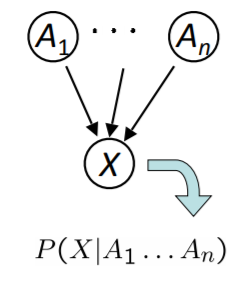
\includegraphics[width=0.25\textwidth]{figs/bayes1.png}
    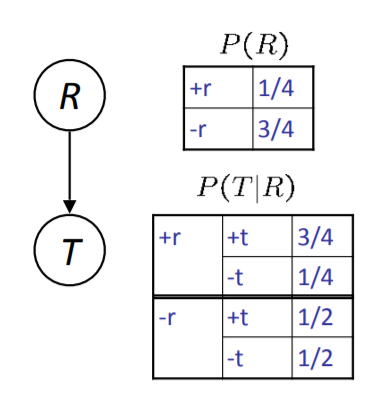
\includegraphics[width=0.25\textwidth]{figs/bayes2.png}
    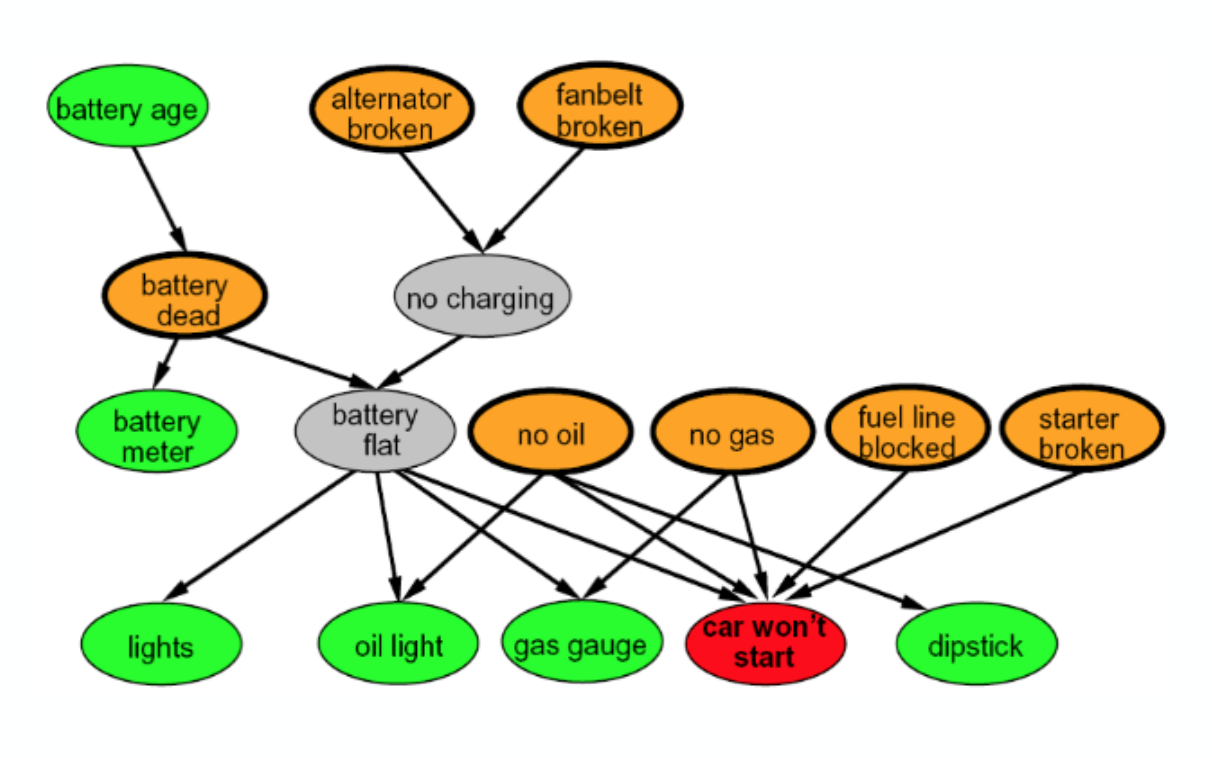
\includegraphics[scale=0.4]{figs/carrepair}
    \caption{Conditional implications example (left), example conditional probability tables (center), and example bayes net for car repair (right)}
    \label{fig:bayes}
\end{figure}

\textbf{Bayes' Nets encode conditional independence.} Just like how the Markov assumption allowed us to simplify equations based on conditional independence across time, the topology of Bayes' Nets can allow us to also assume conditional independence given various pieces of evidence (observed variables). \textbf{D-Separation} is one powerful and simple procedure for determining if $X_i$ and  $X_j$ are conditionally independent given other variables:
\begin{itemize}
    \item Check all undirected paths between $X_i$ and $X_j$
    \item If one or more paths active, then independence not guaranteed (a path is active if each triple is active). Otherwise (i.e. if all paths are inactive), then independence is guaranteed. See Figure~\ref{fig:triples} for the list of active and inactive triples to analyze on each path.
\end{itemize}

\begin{figure}[ht]
    \centering
    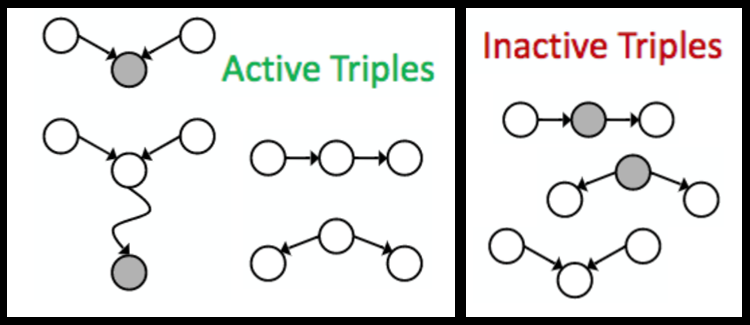
\includegraphics[width=0.6\textwidth]{figs/triples.png}
    \caption{Active and inactive triples for D-Separation. Nodes in grey are assigned. Canonical names for active triples are common effect (left), common cause (bottom right), and causal chain (top right).}
    \label{fig:triples}
\end{figure}

\textbf{Inference} is the process of calculating some resulting quantity from a joint distribution (such as a posterior probability $P(X|E_1=e_1,E_2=e_2)$, or most likely explanation $argmax_x \; P(X=x|E_1=e_1,E_2=e_2)$).
\begin{itemize}
    \item \textbf{Enumeration} is the process of creating the full joint distribution over all of the variables and summing out any unneeded variables. For example if you wanted to determine the probability of the variable $Q$ given evidence $E_1=e_1 \ldots E_k = e_k$ but that also related to other variables $H_1 \ldots H_r$ (canonically called ``hidden variables'') you could:
    \begin{enumerate}
        \item Multiply all factors to construct the full joint distribution:
        $$P(Q, H_1, \dots H_r, E_1, \dots, E_k)$$
        \item Sum out all $H_i$ to get joint of query and evidence (selecting rows consistent with the evidence):
        $$P(Q, e_1 \cdots e_k) = \sum_{h_1 \cdots h_r} P(Q, h_1 \cdots h_r, e_1 \cdots e_k)$$
        \item Normalize across all $Q$:
        $$P(Q=q_k | e_1 \cdots e_k) = \frac{P(Q=q_k, e_1 \cdots e_k)}{\sum_{q_i} P(Q=q_i, e_1 \cdots e_k)}$$
    \end{enumerate}
    This proves to be slow as you have to join up the whole joint distribution over all $Q,H,E=e$ before you sum out the hidden variables.
    \item \textbf{Variable Elimination} is a (usually) faster approach (although still NP-Hard) which interleaves joining and marginalizing over the hidden variables. It relies on computing \textbf{factors} which are simply CPTs where some of the variables are observed (selected, known). The process starts with the initial factors, aka the CPTs selecting the known rows just like in enumeration. However instead of forming the full joint distribution we do (see Figure~\ref{fig:enumvselim} for a high level schematic difference):
    \begin{enumerate}
        \item Pick a hidden variable $H_k$
        \item Join all factors mentioning $H_k$ by forming joint distributions:\\
        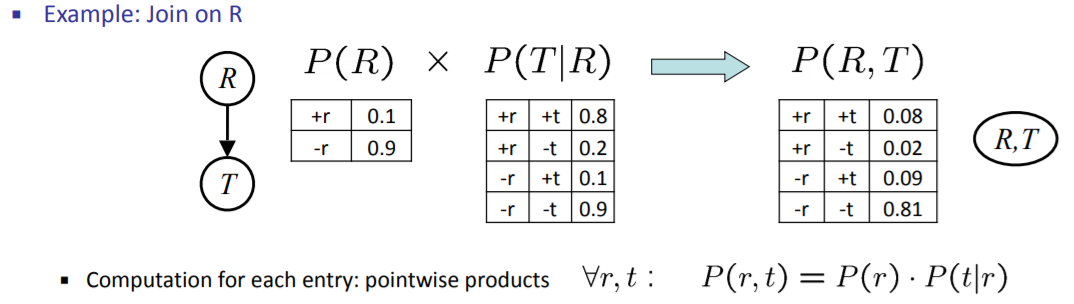
\includegraphics[width=0.8\textwidth]{figs/join.png}
        \item Eliminate (sum out) $H_k$ by computing the marginal distribution:\\
        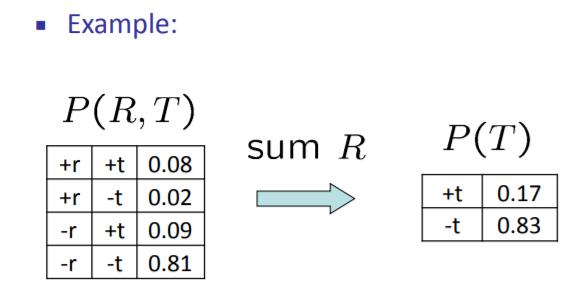
\includegraphics[width=0.4\textwidth]{figs/marginalize.png}
        \item Repeat until all hidden factors are removed. Then do a final join with anything that is left over and normalize!
    \end{enumerate}
    \begin{figure}[ht]
        \centering
        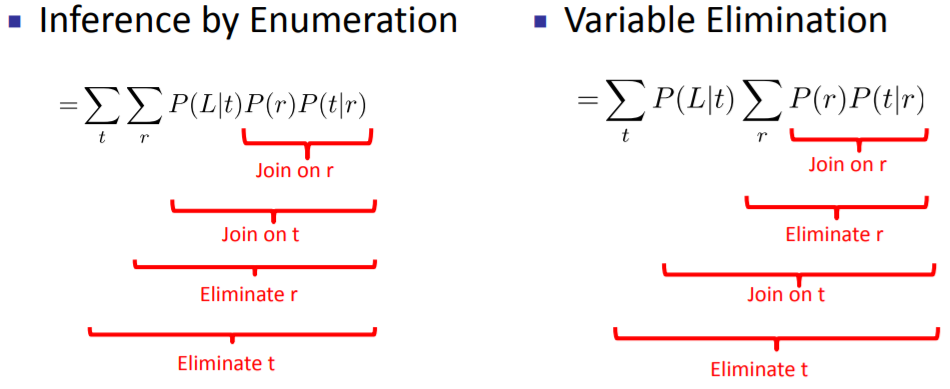
\includegraphics[width=0.6\textwidth]{figs/enumvselim.png}
        \caption{Summary of enumeration vs variable elimination.}
        \label{fig:enumvselim}
    \end{figure}
\end{itemize}

\textbf{Approximate Inference via Sampling}: both Enumeration and Variable Elimination are methods of exact inference (aka you compute the exact answer), but that can be hard as mentioned above. Sampling can be computationally cheaper and provide a very good approximation in many cases (with theoretical guarantees as the number of samples goes to $\infty$). There are a variety of ways to sample:
\begin{itemize}
    \item \textbf{Prior Sampling} is the simplest approach where one simply samples from the CPTs to get a list of samples. Then one can simply use this list to compute approximate probabilities via counting. This is very fast but does not take into account the inference problem we are trying to solve and is simply trying to sample the full joint distribution.
    \item \textbf{Rejection Sampling} modifies Prior Sampling by rejecting any samples that are irrelevant for our inference problem. This allows us to only have to store in memory and compute over the relevent samples. For example if we condition on $E_1 = 0$ (e.g., we are trying to compute $P(Q|E_1 = 0)$) then all samples with $E_1 \neq 0$ can be rejected. Unfortunately, this may reject many many samples.
    \item \textbf{Likelihood Weighting} reduces the number of wasted samples by fixing the evidence variables and then sampling the rest of the distribution. Importantly (to remain consistent) it weights these samples by their likelihood of occurring. Note: evidence only effects ``downstream'' variables from it.
    $$w(Q,E_1 = e_1) = \prod P(e_1 | \text{Parents}(E)) $$
    \item \textbf{Gibbs Sampling} improves Likelihood Weighting by constructing weights that take into account both upstream and downstream evidence through a process known as Markov Chain Monte Carlo (MCMC). You don't need to know this in detail.
\end{itemize}
%%%%%%%%%%%%%%%%%%%%%%%%%%%%%%%%%%%%%%%%%%%%%%%%%%%%%%%%%%%%%%%%%%%%%%%%%%%%%%%%
%%%%%%%%%%%%%%%%%%%%%%%%%%%%%%%%%%%%%%%%%%%%%%%%%%%%%%%%%%%%%%%%%%%%%%%%%%%%%%%%
\section*{Exercises:}
\begin{enumerate}
    \item Given the following Bayes' Net and CPT, calculate the joint distribution table:\\
    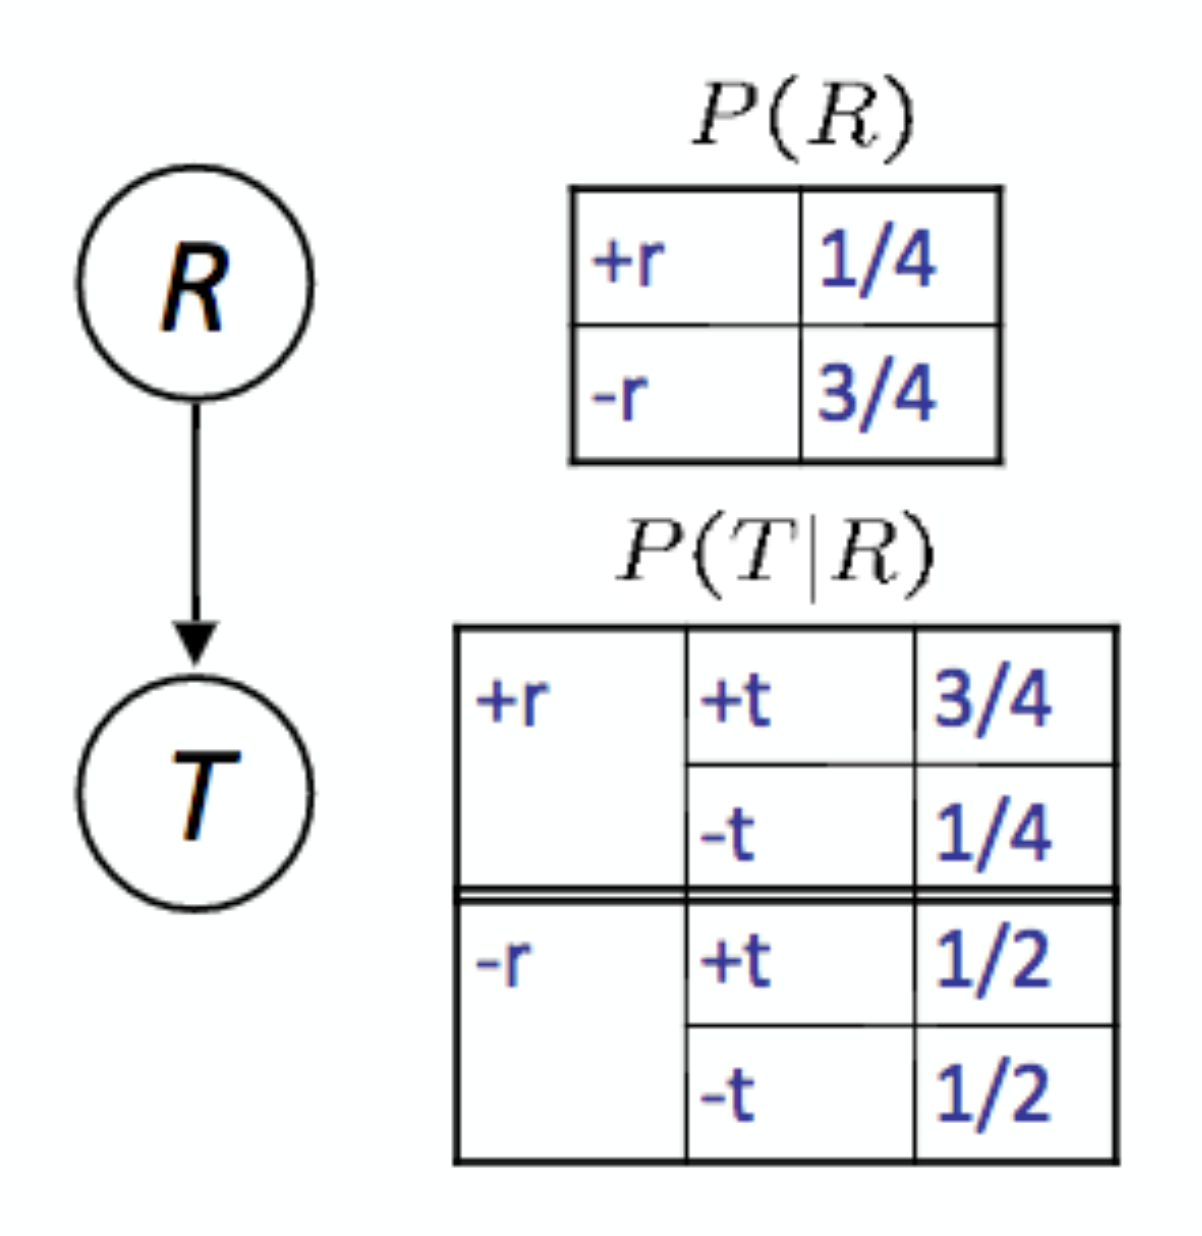
\includegraphics[scale=0.25]{figs/conditional.png} \quad \quad \quad \quad \quad \quad
    \ifsol
        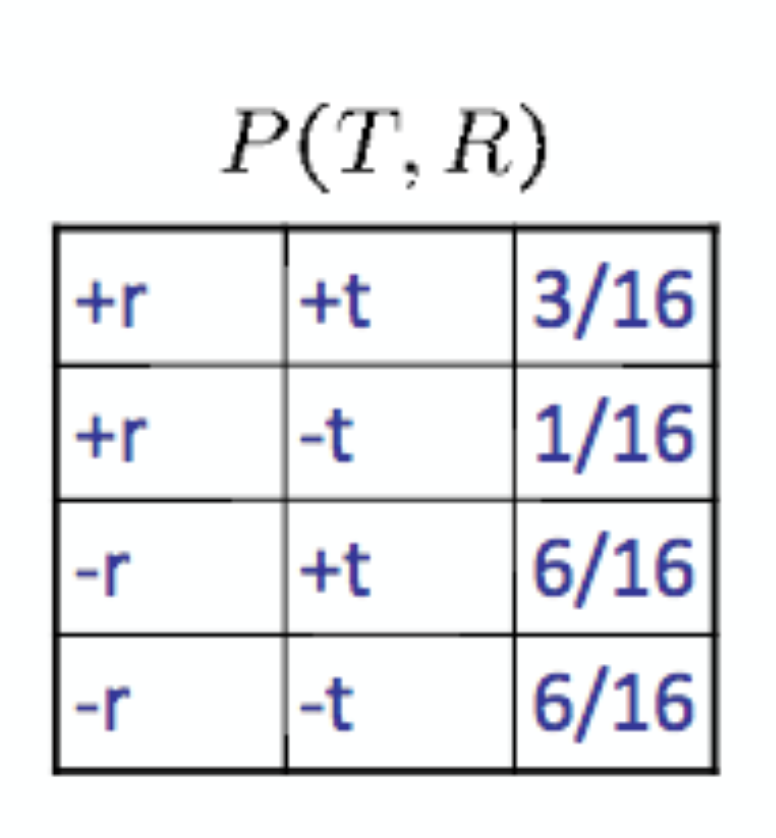
\includegraphics[scale=0.25]{figs/joint.png}
    \fi
    \item Given this Bayes' Net, answer the following questions: \\
    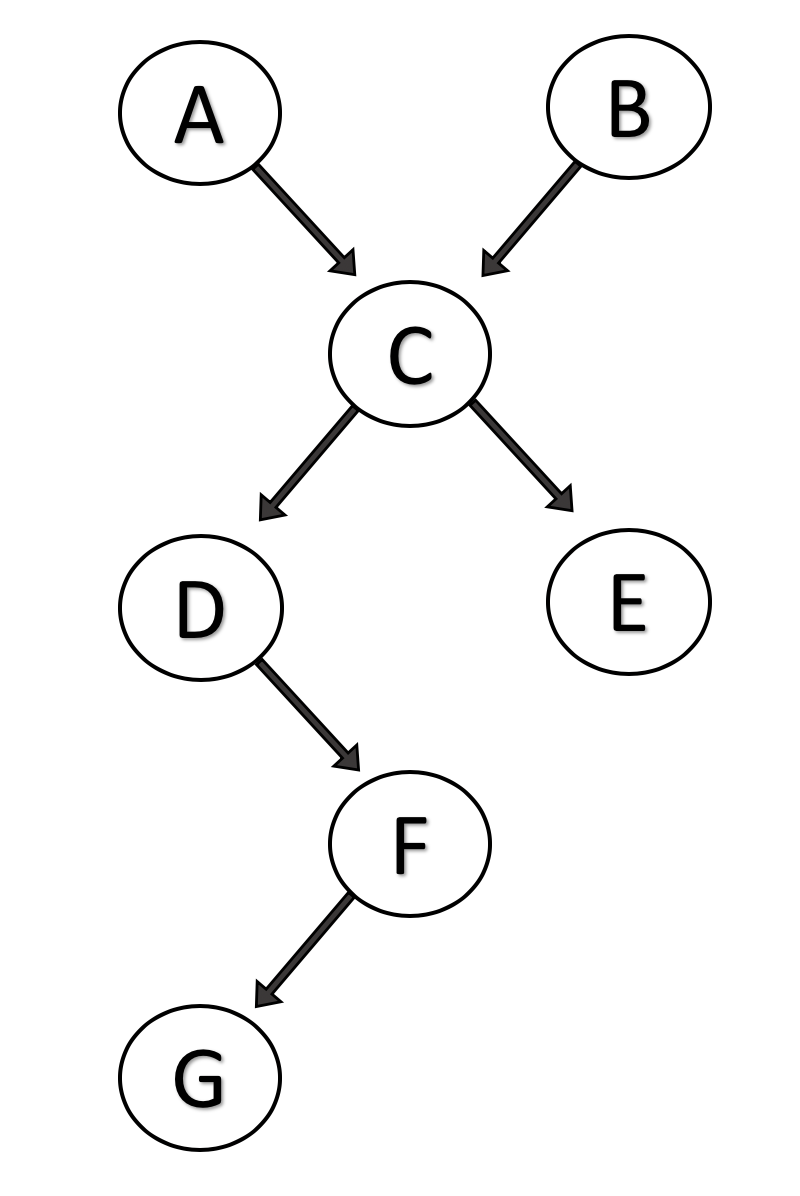
\includegraphics[width=0.18\textwidth]{figs/net1}
    \begin{enumerate}[a)]
        \item  Are A and B conditionally independent, given D and F?\\
            \ifsol
                {\color{blue} No due to common effect (long one)}
            \else
                \vspace{1pt}
            \fi
        \item  Are A and B conditionally independent, given C?\\
            \ifsol
                {\color{blue} No due to common effect (short one)}
            \else
                \vspace{1pt}
            \fi
        \item  Are D and E conditionally independent, given C?\\
            \ifsol
                {\color{blue} Yes}
            \else
                \vspace{1pt}
            \fi
        \item  Are D and E marginally independent (aka with nothing conditioned on)?\\
            \ifsol
                {\color{blue} No due to common cause}
            \else
                \vspace{1pt}
            \fi
    \end{enumerate}
    \newpage
    \item For this Bayes’ net, we are given the query $P(Y | +z)$. All variables have binary domains. \\
    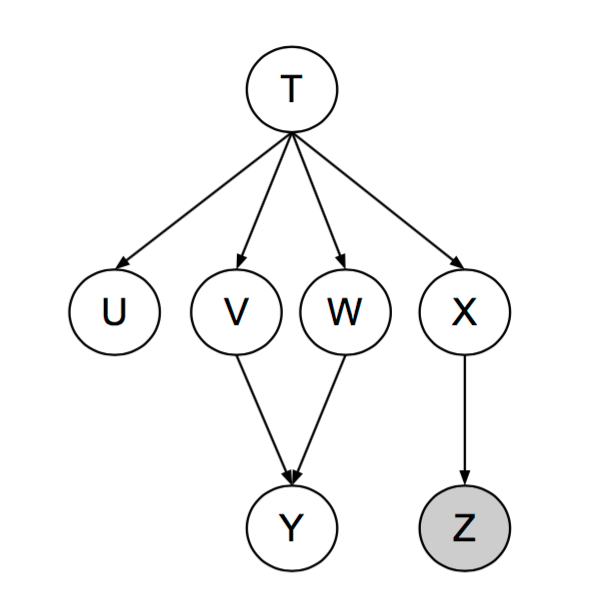
\includegraphics[scale=0.4]{figs/elimnet}\\
    We can solve this via enumeration by computing:
    $$P(Y|+z) = \sum_t \sum_u \sum_v \sum_w \sum_x P(T)P(U|T)P(V|T)P(W|T)P(X|T)P(Y|V,W)P(+z|X)$$
    However, as we know this is often very slow so instead we will use variable elimination to with the following variable elimination ordering: $X, T, U, V, W$.
    \begin{enumerate}[a)]
        \item After inserting evidence, what are the initial factors?\\
        \ifsol
            {\color{blue} $P(T),P(U|T),P(V|T),P(W|T),P(X|T),P(Y|V,W),P(+z|X)$}
        \else
            \vspace{1pt}
        \fi
        \item Eliminating X generates what new factor $f_1$?\\
        \ifsol
            {\color{blue} $f_1(T, +z) =  \sum_x P (x|T )P (+z|x)$}
        \else
            \vspace{1pt}
        \fi
        \item This leaves us with what factors?\\
        \ifsol
            {\color{blue} $P(T),P(U|T),P(V|T),P(W|T),P(Y|V,W),f_1(T,+z)$}
        \else
            \vspace{1pt}
        \fi
        \item Eliminating T generates what new factor $f_2$?\\
        \ifsol
            {\color{blue} $f_2(U,V,W,+z) =  \sum_t P(t)P(U|t)P(V |t)P(W|t)f_1(t,+z)$}
        \else
            \vspace{1pt}
        \fi
        \item This leaves us with what factors?\\
        \ifsol
            {\color{blue} $P(Y|V,W),f_2(U,V,W,+z)$}
        \else
            \vspace{1pt}
        \fi
        \item Eliminating U generates what new factor $f_3$?\\
        \ifsol
            {\color{blue} $f_3(V,W,+z) = \sum_u f_2(u,V,W,+z)$}
        \else
            \vspace{1pt}
        \fi
        \item This leaves us with what factors?\\
        \ifsol
            {\color{blue} $P(Y|V,W),f_3(V,W,+z)$}
        \else
            \vspace{1pt}
        \fi
        \item Eliminating V generates what new factor $f_4$?\\
        \ifsol
            {\color{blue} $f_4(W, Y, +z) =  \sum_v f_3(v, W, +z)P (Y |v, W )$}
        \else
            \vspace{1pt}
        \fi
        \item This leaves us with what factors?\\
        \ifsol
            {\color{blue} $f_4(W,Y,+z)$}
        \else
            \vspace{1pt}
        \fi
        \item Finally eliminating Y generates what new factor $f_5$?\\
        \ifsol
            {\color{blue} $f_5(Y, +z) =  \sum_w f_4(w, Y, +z)$}
        \else
            \vspace{1pt}
        \fi
        \item How would you obtain $P(Y | +z)$ from the remaining factors?\\
        \ifsol
            {\color{blue} Well we only have one factor left so simply renormalize $f_5(Y, +z)$ to obtain $P (Y | +z)$. $$P(y|+z)= \frac{f_5(y,+z)}{\sum_{y'} f_5(y',+z)}$$}
        \else
            \vspace{2pt}
        \fi
        \item What is the size of the largest factor that gets generated during the above process? Does there exist a better elimination ordering (one which generates smaller largest factors)?\\
        \ifsol
            {\color{blue} $f_2(U, V, W, +z)$, which has $3$ binary variables, has size $2^3 = 8$. Yes, elimination ordering of $X , U , T , V , W$ generates only factors of up to size $2^2 = 4$.}
        \else
            \vspace{2pt}
        \fi
    \end{enumerate}
    \clearpage
    \item Suppose you are given the following Bayes net and conditional probability distributions:
    \begin{figure}[ht]
        \centering
        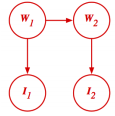
\includegraphics[width=.1\textwidth]{figs/graphical}
        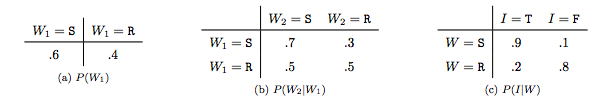
\includegraphics[width=.7\textwidth]{figs/tables}
    \end{figure}
    This is sufficient to specify a joint probability distribution for the four variables. We want to do approximate inference through sampling. We sample and produce the following samples for $(W_1, I_1, W_2, I_2)$:
    \begin{figure}[h]
        \centering
        \vspace{-1em}
        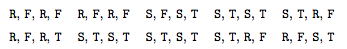
\includegraphics[width=.55\textwidth]{figs/samples}
        \vspace{-2em}
    \end{figure}
    \begin{enumerate}[a)]
        \item What is $\hat{P}(W_2=R)$, the probability that sampling assigns to the event $W_2 = R$?\\
        \ifsol
            \textcolor{blue}{$W_2 = R$ in 5 of the 10 samples, therefore the probability is 0.5.}
        \else
            \vspace{2em}
        \fi
        \item Cross of samples rejected by rejection sampling if we are computing $P(W_2|I_1=T, I_2=F)$\\
        \ifsol
            \begin{figure}[h]
                \centering
                \vspace{-1em}
                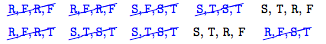
\includegraphics[width=.55\textwidth]{figs/crossed-off}
                \vspace{-1.5em}
            \end{figure}
        \else
            \begin{figure}[h]
                \centering
                \vspace{-1em}
                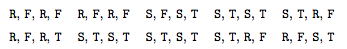
\includegraphics[width=.55\textwidth]{figs/samples}
                \vspace{-1.5em}
            \end{figure}
        \fi
    \end{enumerate}
    Rejection sampling seems to be wasting a lot of effort, so we decide to use likelihood weighting instead. Assume we generate the following six samples given the evidence $I_1 = T$ and $I_2 = F$:
    \begin{figure}[h!]
        \centering
        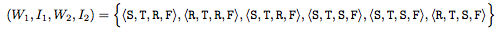
\includegraphics[width=.7\textwidth]{figs/samplelist}
    \end{figure}\\
    Recall that in likelihood weighting, we give weight to a sample according to:
    \[
    \prod_{\text{Evidence variables } e} P(e|\text{Parents}(e))
    \]
    \begin{enumerate}[c)]
        \item What is the weight of the first sample $(S,T,R,F)$?\\
        \ifsol
            \textcolor{blue}{The evidence is $I_1 = T, I_2 = F$. The weight of the first sample is therefore:
            $$w = P(I_1=T|W_1=S) \cdot P(I_2=F|W_2=R) = 0.9 \cdot 0.8 = 0.72$$}
            \vspace{-1em}
        \else
            \vspace{2em}
        \fi
    \end{enumerate}
    \begin{enumerate}[d)]
        \item Use likelihood weighting to estimate $\hat{P}(W_2|I_1=T,I_2=F$\\
        \ifsol
            \textcolor{blue}{The sample weights are shown in in the following table:
            \begin{figure}[h!]
            \centering
            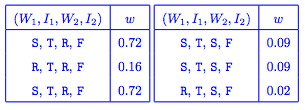
\includegraphics[width=.35\textwidth]{figs/soltable}
            \end{figure}\\
            To compute the probabilities, we normalize the weights and find that:
            \begin{equation*}
                \begin{split}
                \hat{P}(W_2=R|I_1=T,I_2=F) &= \frac{0.72+0.16+0.72}{0.72+0.16+0.72+0.09+0.09+0.02} = 0.889 \\    \hat{P}(W_2=S|I_1=T,I_2=F) &= 1-0.889 =  0.111 
                \end{split}
            \end{equation*}}
        \else
            \vspace{2em}
        \fi
    \end{enumerate}
\end{enumerate}
\end{document}
